\section{Convex problems}
\subsection{Optimization problems in standard form}
\begin{definition}[Optimization problem]
    In its standard form, an optimization problem can be written as:
    \begin{equation*}
        \text{minimize } f(x) \quad\text{subject to}\quad \begin{cases}
            \forall i\in\iset{1}{m}, \quad g_i(x)\leq 0\\
            \forall j\in\iset{1}{p}, \quad h_j(x) = 0
        \end{cases}
    \end{equation*}
    where:
    \begin{itemize}
        \item $x\in\R^n$ is the optimization variable
        \item $f:\R^n\to\R$ is the \emph{objectif} or \emph{cost function}
        \item $g_i:\R^n\to\R$ are the inequality constraint functions
        \item $h_j:\R^n\to\R$ are the equality constraint functions
    \end{itemize}
\end{definition}
\begin{remark}
    This form can be generalized to support an infinity of constraints, and strict inequalities. Note that we can assume that the problem is subject only to inequations, without loss of generality: indeed, each equality $h_i(x)=0$ can be expressed as two inequations $h_i(x)\leq0$ and $-h_i(x)\leq0$.
\end{remark}

\begin{definition}[Optimal value]
    We define the optimal value associated to this optimization problem as:
    \begin{equation*}
        p^* := \inf\set{f(x)}{\forall i\in\iset{1}{m}, \: g_i(x)\leq 0 \quad\text{and}\quad \forall j\in\iset{1}{p}, \: h_j(x) = 0}
    \end{equation*}
    If $p^*=+\infty$, the problem is \say{infeasible}: no $x$ satisfies the constraints.\\
    If $p^*=-\infty$, the problem is \emph{unbounded below}.
\end{definition}

\begin{remark}
    An optimization problem in standard form has an \emph{implicit constraint} defined by the domain of the constraint functions:
    \begin{equation*}
        x\in\D := \bigcap_{i=0}^m\dom g_i \cap \bigcap_{j=0}^p\dom h_j
    \end{equation*}
    We call $\D$ the \emph{domain of the problem}. The constraints $g_i(x)\leq0$ and $h_j(x)=0$ are the explicit constraints, and the domain of the problem defines the implicit constraints. A problem is \emph{unconstrained} if it has no explicit constraints ($m=p=0$).
\end{remark}

\begin{example}
    The following problem is unconstrained:
    \begin{equation*}
        \text{minimize } -\sum_{i=1}^k\log(b_i-a_i^\tp x)
    \end{equation*}
    The implit constraints are $a_i^\tp x<b_i$ for all $i\in\iset{1}{k}$.
\end{example}

\begin{definition}[Feasibility problem]
    A feasibility problem is an optimization problem in which we seek a feasible point, i.e. a point that satisfies the constraints. It can be written as:
    \begin{equation*}
        \text{find } x \quad\text{subject to}\quad \begin{cases}
            \forall i\in\iset{1}{m}, \quad g_i(x)\leq 0\\
            \forall j\in\iset{1}{p}, \quad h_j(x) = 0
        \end{cases}
    \end{equation*}
    It can be considered a special case of the general problem with $f(x)=0$:
    \begin{equation*}
        \text{minimize } 0 \quad\text{subject to}\quad \begin{cases}
            \forall i\in\iset{1}{m}, \quad g_i(x)\leq 0\\
            \forall j\in\iset{1}{p}, \quad h_j(x) = 0
        \end{cases}
    \end{equation*}
    If constraints are feasible, $p^*=0$ and any feasible $x$ is optimal.\\
    If constraints are infeasible, $p^*=+\infty$.
\end{definition}

\subsection{Convex optimization problems}
\subsubsection{Definition}
\begin{definition}[Convex Optimization problem]
    \label{def:convex-optimization-problem}
    In its standard form, a convex optimization problem can be written as:
    \begin{equation*}
        \text{minimize } f(x) \quad\text{subject to}\quad \begin{cases}
            \forall i\in\iset{1}{m}, \quad g_i(x)\leq 0\\
            \forall j\in\iset{1}{p}, \quad a_j^\tp x = b_j
        \end{cases}
    \end{equation*}
    where the $g_i$ are convex, and the equality constraints are affine.

    Such a problem is often written as:
    \begin{equation*}
        \text{minimize } f(x) \quad\text{subject to}\quad \begin{cases}
            \forall i\in\iset{1}{m}, \quad g_i(x)\leq 0\\
            Ax = b
        \end{cases}
    \end{equation*}
\end{definition}

\begin{remark}
    The feasible set of a convex optimization problem is convex.
\end{remark}

\begin{example}
    Consider the following optimization problem:
    \begin{equation*}
        \text{minimize } x_1^2 + x_2^2 \quad\text{subject to}\quad \begin{cases}
            g_1(x) = x_1/(1+x_2^2) \leq 0\\
            h_1(x) = (x_1+x_2)^2 = 0
        \end{cases}
    \end{equation*}
    The objective function $f(x)=x_1^2+x_2^2$ is convex, and the feasible set
    \begin{equation*}
        \set{(x_1, x_2)}{x_1=-x_2\leq0}
    \end{equation*}
    is convex. Nevertheless, this is not a convex problem according to Definition \ref{def:convex-optimization-problem} because the constraint $g_1(x)$ is not convex and $h_1$ is not affine. We can rewrite this problem in an equivalent but not identical form:
    \begin{equation*}
        \text{minimize } x_1^2 + x_2^2 \quad\text{subject to}\quad \begin{cases}
            x_1\leq0\\
            x_1+x_2=0
        \end{cases}
    \end{equation*}
    This problem is now convex according to Definition \ref{def:convex-optimization-problem}.
\end{example}

\begin{remark}
    One could ask why we enforce this definition for a convex optimization problem, and why we do not open it to more general forms. In general, recognizing a convex optimization problem is a difficult task, and this allows to provide a simple definition that is easy to check. Note that software tools exist to recognize convex optimization problems via composition rules, such as \emph{Disciplined Convex Programming (DCP)}.
\end{remark}

\subsubsection{Optimal and locally optimal points}
\begin{definition}[Feasible point]
    A point $x$ is \emph{feasible} if $x\in\dom f$ and it satisfies the constraints:
    \begin{equation*}
        \forall i\in\iset{1}{m}, \: g_i(x)\leq0 \quad\text{and}\quad \forall j\in\iset{1}{p}, \: h_j(x)=0
    \end{equation*}
\end{definition}

\begin{definition}[Optimal point]
    A feasible point $x$ is \emph{optimal} if $f(x)=p^*$. We denote $X_{\text{opt}}$ the set of optimal points.
\end{definition}

\begin{definition}[Locally optimal point]
    A point $x$ is \emph{locally optimal} if there is an $R>0$ such that $x$ is optimal for the problem restricted to the ball $B(x, R)$:
    \begin{equation*}
        \text{minimize } f(z) \quad\text{subject to}\quad \begin{cases}
            \forall i\in\iset{1}{m}, \quad g_i(x)\leq 0\\
            \forall j\in\iset{1}{p}, \quad h_j(z) = 0\\
            \norm{z-x}_2\leq R
        \end{cases}
    \end{equation*}
\end{definition}

\begin{example}
    With $n=1, m=p=0$:
    \begin{itemize}
        \item $f(x)=x\log x$, we have $\dom f=\R_+^*$, $p^*=-1/e$, and $x=1/e$ is optimal
        \item $f(x)=1/x$, we have $\dom f=\R_+^*$, $p^*=0$, but no optimal point
        \item $f(x)=-\log x$, we have $\dom f=\R_+^*$, $p^*=-\infty$
        \item $f(x)=x^3-3x$, we have $p^*=-\infty$ but a local optimum at $x=1$
    \end{itemize}
\end{example}

\begin{theorem}[Global optimality for convex problems]
    Any locally optimal point of a convex problem is globally optimal.
\end{theorem}
\begin{proof}
    Suppose that $x$ is locally optimal and $y$ is optimal with $f(y)<f(x)$. Since $x$ is locally optimal, there is an $R>0$ such that:
    \begin{equation*}
        \forall z\in B(x, R), \quad z\text{ feasible} \implies f(z)\geq f(x)
    \end{equation*}
    Now consider $z=\theta y + (1-\theta)x$ with $\theta=R/(2\norm{y-x}_2)$. Since $\norm{y-x}_2>R$, we must have $0<\theta<1/2$. $z$ is a combination of two feasible points, hence it is feasible since the problem is convex. Finally, $\norm{z-x}_2=R/2$ hence $z\in B(x, R)$, and:
    \begin{equation*}
        f(z)\leq\theta f(x)+(1-\theta)f(y)<f(x)
    \end{equation*}
    which contradicts the assumption that $x$ is locally optimal.
\end{proof}

\subsubsection{Equivalent convex problems}
Two problems are informally equivalent if the solution of one is readily obtained from the solution of the other, and vice-versa. In the following, we will see multiple transformations that preserve both the solution and the convexity of an optimization problem.

\paragraph*{Eliminating equality constraints}
Consider the problem:
\begin{equation*}
    \text{minimize } f(x) \quad\text{subject to}\quad \begin{cases}
        \forall i\in\iset{1}{m}, \quad g_i(x)\leq 0\\
        Ax = b
    \end{cases}
\end{equation*}
If we can find $F$ and $x_0$ such that:
\begin{equation*}
    Ax=b \iff \exists z, \: x=Fz+x_0
\end{equation*}
then we can rewrite the problem as:
\begin{equation*}
    \text{minimize } f(Fz+x_0) \quad\text{subject to}\quad \forall i\in\iset{1}{m}, \: g_i(Fz+x_0)\leq 0
\end{equation*}
For instance, one can choose $F$ such that $\im(F)=\Ker(A)$ and $x_0$ such that $Ax_0=b$.

\paragraph*{Introducing equality constraints}
Reciprocally, the problem:
\begin{equation*}
    \text{minimize } f(A_0z+b_0) \quad\text{subject to}\quad \forall i\in\iset{1}{m}, \: g_i(A_iz+b_i)\leq 0
\end{equation*}
Can be rewritten as:
\begin{equation*}
    \text{minimize } f(y_0) \quad\text{subject to}\quad \begin{cases}
        \forall i\in\iset{1}{m}, \quad g_i(y_i)\leq 0\\
        \forall i\in\iset{0}{m}, \quad y_i=A_ix+b_i
    \end{cases}
\end{equation*}

\paragraph*{Introducing slack variables for linear inequalities}
The idea is to replace linear inequalities by linear equalities and non-negativity constraints.
Formally, the problem:
\begin{equation*}
    \text{minimize } f(x) \quad\text{subject to}\quad \forall i\in\iset{1}{m}, \: a_i^\tp x\leq b_i
\end{equation*}
is equivalent to:
\begin{equation*}
    \text{minimize } f(y_0) \quad\text{subject to}\quad \begin{cases}
        \forall i\in\iset{1}{m}, \: a_i^\tp x + s_i = b_i\\
        \forall i\in\iset{1}{m}, \: s_i\geq0
    \end{cases}
\end{equation*}

\paragraph*{Epigraph form}
We saw previously that the epigraph of a convex function is a convex set. We can use this property to rewrite a convex optimization problem in its standard form as:
\begin{equation*}
    \text{minimize } t \quad\text{subject to}\quad \begin{cases}
        f(x)-t\leq0\\
        \forall i\in\iset{1}{m}, \: g_i(x)\leq 0\\
        Ax=b
    \end{cases}
\end{equation*}

\paragraph*{Minimizing over some variables}
Consider the problem:
\begin{equation*}
    \text{minimize } f(x_1, x_2) \quad\text{subject to}\quad \forall i\in\iset{1}{m}, \: g_i(x_1)\leq 0
\end{equation*}
This can be rewritten as:
\begin{equation*}
    \text{minimize } \tilde{f}(x_1) \quad\text{subject to}\quad \forall i\in\iset{1}{m}, \: g_i(x_1)\leq 0\\
\end{equation*}
where $\tilde{f}(x_1)=\inf_{x_2}f(x_1, x_2)$. Said otherwise, we can start by minimizing over the unconstrained variables, and then minimize over the constrained variables.

\subsection{Special classes of convex problems}
If methods exist to solve general convex optimization problems, some classes of problems have specific structures that can be exploited to design more efficient algorithms. We will present some of these classes in the following.

\subsubsection{Linear programming (LP)}
\begin{definition}[Linear programming problem]
    A linear programming problem is an optimization problem in which the objective function is affine and the constraints are linear:
    \begin{equation*}
        \text{minimize } c^\tp x + d\quad\text{subject to}\: \begin{cases}
            Gx\leq h\\
            Ax=b
        \end{cases}
    \end{equation*}
    The feasible set of a linear programming problem is a polyhedron $\Pc$.
    \begin{figure}[H]
        \centering
        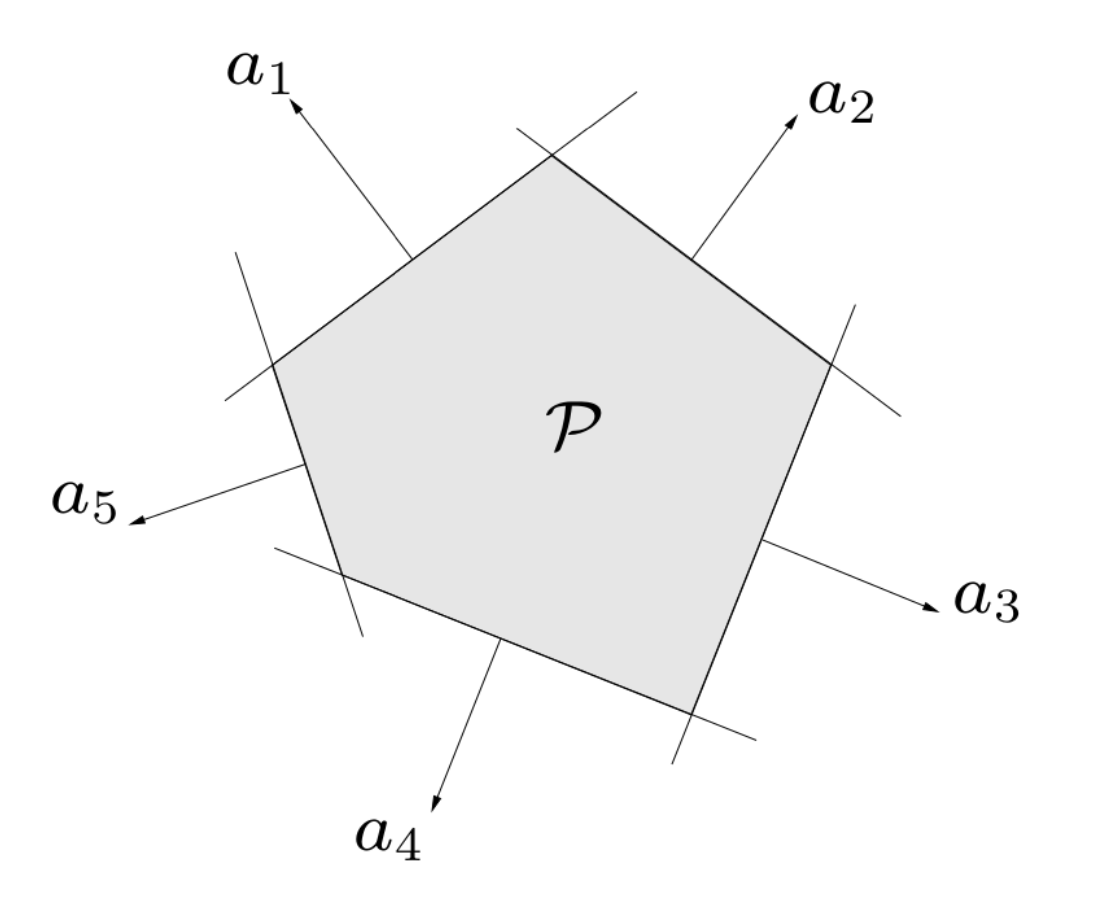
\includegraphics[width=.5\textwidth]{convex-problems/polyhedron.png}
        \caption{A polyhedron $\Pc$, the feasible set of a linear programming problem.}
    \end{figure}
\end{definition}

As an example, we consider the problem of finding the Chebyshev center of a polyhedron.
\begin{definition}[Chebyshev center]
    Given a polyhedron $\Pc$ of the form:
    \begin{equation*}
        \Pc = \set{x}{\forall i\in\iset{1}{m}, \: a_i^\tp x\leq b_i,}
    \end{equation*}
    its \emph{Chebyshev center} is the center of the largest inscribed ball. Recall that the ball $B(x_c, r)$ of center $x_c$ and radius $r$ is defined as:
    \begin{equation*}
        B(x_c, r) = \set{x}{\norm{x-x_c}_2\leq r}
    \end{equation*}
    Then, the Chebyshev center $\hat{x}$ is the point $x_c$ that maximizes $r$:
    \begin{equation*}
        \hat{x} = \argmin_{x_c, r} \set{r\in\R_+}{B(x_c, r)\subseteq\Pc} = \argmin_{x_c} \max_{x\in\Pc} \norm{x-x_c}_2
    \end{equation*}
\end{definition}

\begin{property}[Chebyshev center as a linear programming problem]
    The Chebyshev center of a polyhedron $\Pc$ can be computed as the solution of the following linear programming problem:
    \begin{equation*}
        \text{maximize } r \quad\text{subject to}\quad \forall i\in\iset{1}{m}, \: a_i^\tp x_c + r\norm{a_i}_2\leq b_i
    \end{equation*}
\end{property}

\subsubsection{Convex quadratic programming (QP)}

\subsubsection{Quadratically constrained quadratic programming (QCQP)}

\subsubsection{Second-order cone programming (SOCP)}

\subsection{Robust linear programming}
\subsubsection{Deterministic approach via SOCP}
\subsubsection{Stochastic approach via SOCP}

\subsection{Generalized inequalities}